\chapter{Experimental Results and Comparative Analysis}

\section{Training Dynamics and Convergence Behavior}

Figure 6.1 illustrates the training and validation loss trajectories for both the proposed Swin Transformer framework and the baseline ResNet-50 + LSTM architecture on the ROCOv2 training corpus (59,958 images).

\begin{figure}[!htbp]
\centering
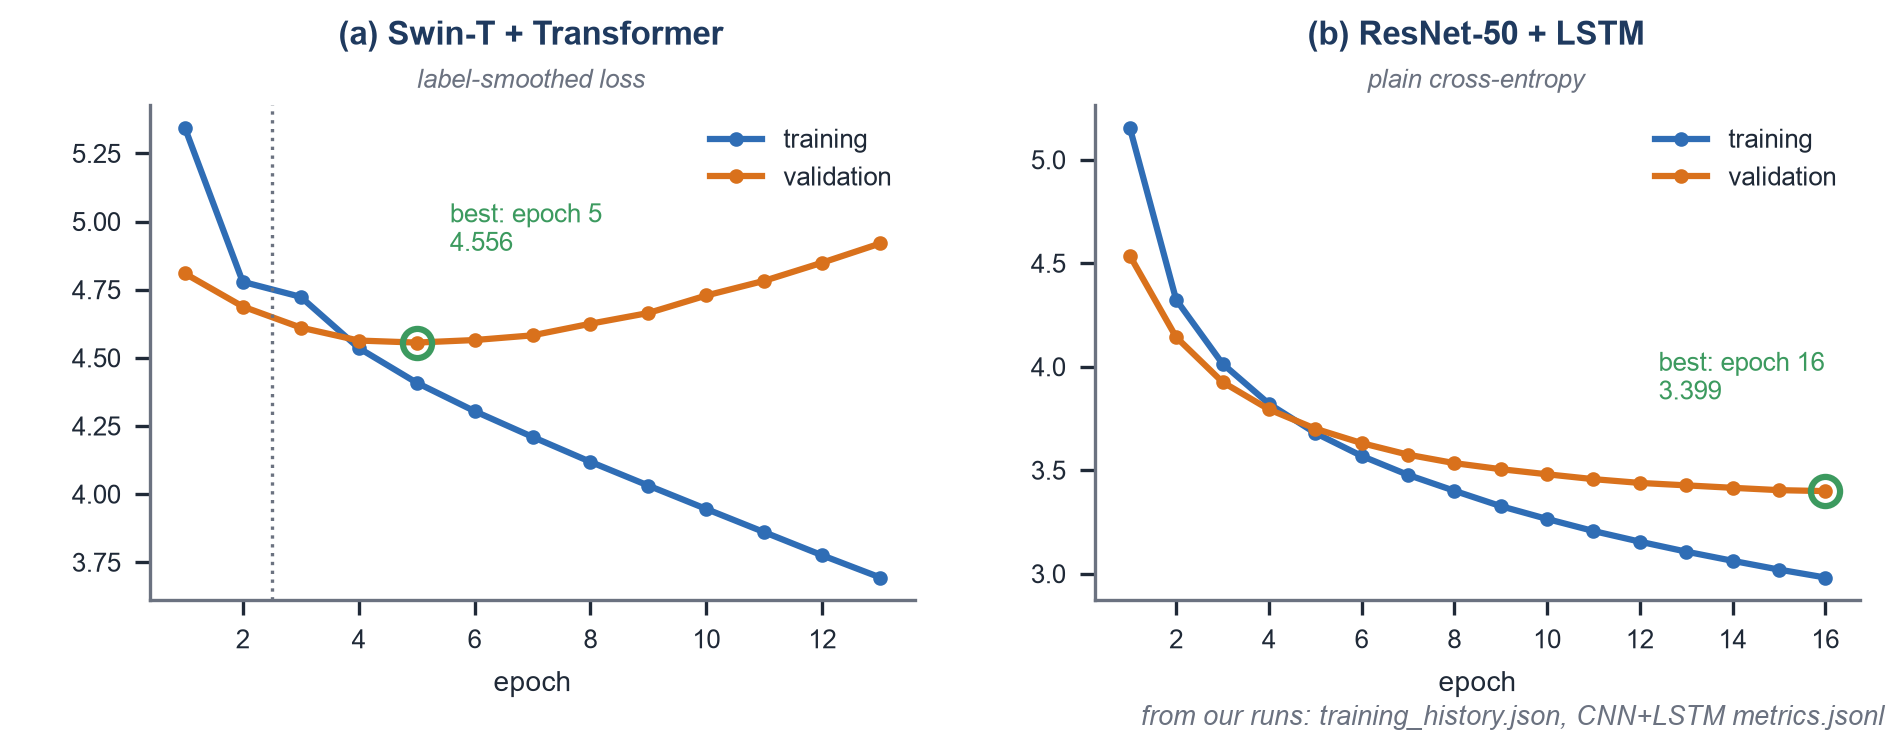
\includegraphics[width=0.95\linewidth,height=\textheight,keepaspectratio]{figures/fig6_1_loss_curves.png}
\caption{Training and validation loss trajectories. (a) Swin-T + Transformer: Phase 1 (epochs 1--2) warms up the decoder while freezing the encoder; Phase 2 (epochs 3--13) unfreezes the encoder end-to-end, achieving optimal validation loss of \textbf{4.556 at epoch 5} before early stopping triggers. (b) ResNet-50 + LSTM baseline trained steadily over 16 epochs.}
\end{figure}

\begin{itemize}
\item \textbf{Swin Transformer Architecture:} During Phase 1 (epochs 1--2), the Swin visual encoder remains frozen while the 6-layer Transformer decoder adapts its cross-attention weights to ImageNet visual representations, reducing validation loss from 4.809 to 4.688. In Phase 2, end-to-end fine-tuning with differential learning rates ($1.5 \times 10^{-5}$ for the backbone, $1.0 \times 10^{-4}$ for the decoder) drives the validation loss to an optimal minimum of \textbf{4.556 at epoch 5}. Beyond epoch 5, validation loss slowly diverges while training loss continues to fall, indicating the onset of capacity memorization. Early stopping automatically halted execution at epoch 13, and the epoch 5 checkpoint is preserved as the definitive production model.
\item \textbf{CNN + LSTM Baseline:} The baseline shows monotonic cross-entropy descent, reaching a validation loss of 3.399 at epoch 16. Direct numeric comparison between raw loss values is uninformative, as the Swin loss incorporates label smoothing ($\epsilon = 0.10$), which imposes a theoretical floor on loss, and the two models operate over distinct vocabulary sizes (8,729 vs.\ 8,000 tokens).
\end{itemize}

\section{Head-to-Head Test Split Benchmark (9,927 Images)}

To guarantee an unbiased, rigorous empirical assessment, both models were benchmarked on the complete, uncurated \textbf{ROCOv2 test split} ($N = 9{,}927$ images) under identical hardware and pipeline conditions using an NVIDIA GeForce RTX 4060 Laptop GPU (CUDA 11.8, PyTorch AMP FP16, batch size 8). Table 6.1 summarizes the quantitative performance across all standard n-gram precision (BLEU-1..4), structural sequence recall (ROUGE-L), consensus TF-IDF overlap (CIDEr-D), token classification accuracy, and caption diversity metrics.

\needspace{16\baselineskip}

\begin{table}[!htbp]
\centering
\small
\caption{Comprehensive quantitative evaluation on the full ROCOv2 test set (9,927 images). Bold values indicate superior performance.}
\begin{tabular}{@{}lcccc@{}}
\toprule
\textbf{Metric} & \textbf{ResNet-50 + LSTM} & \textbf{Swin-T (Greedy)} & \textbf{Swin-T (Beam $k=4$)} & \textbf{Relative Gain} \\
\midrule
\textbf{Parameters (Total)} & 35.38 M & 90.94 M & 90.94 M & $+157.0\%$ \\
\quad \textendash\ \textit{Encoder / Decoder} & 24.56 M / 10.83 M & 27.52 M / 63.42 M & 27.52 M / 63.42 M & --- \\
\midrule
\textbf{BLEU-1} & 0.1571 & \textbf{0.1716} & \textbf{0.1833} & $+16.7\%$ \\
\textbf{BLEU-2} & 0.0871 & \textbf{0.0984} & \textbf{0.1099} & $+26.2\%$ \\
\textbf{BLEU-3} & 0.0482 & \textbf{0.0561} & \textbf{0.0644} & $+33.6\%$ \\
\textbf{BLEU-4} & 0.0273 & \textbf{0.0327} & \textbf{0.0379} & $+38.8\%$ \\
\textbf{ROUGE-L} & 0.1831 & \textbf{0.2033} & \textbf{0.2160} & $+18.0\%$ \\
\textbf{CIDEr-D} & 0.1726 & \textbf{0.2171} & \textbf{0.3438} & $+99.2\%$ \\
\midrule
\textbf{Token Accuracy (Lexical)} & 31.67\% & \textbf{32.54\%} & --- & $+2.7\%$ \\
\textbf{Distinct Caption Rate} & 43.98\% & \textbf{52.27\%} & \textbf{79.80\%} & $+81.4\%$ \\
\midrule
\textbf{Model Compute Latency} & \textbf{7.98 ms} & 40.52 ms & 45.20 ms & --- \\
\textbf{Throughput (incl.\ I/O)} & \textbf{63.70 img/s} & 20.30 img/s & 18.20 img/s & --- \\
\textbf{Peak GPU Memory} & \textbf{0.53 GiB} & 0.91 GiB & 1.05 GiB & --- \\
\bottomrule
\end{tabular}
\end{table}

\begin{figure}[!htbp]
\centering
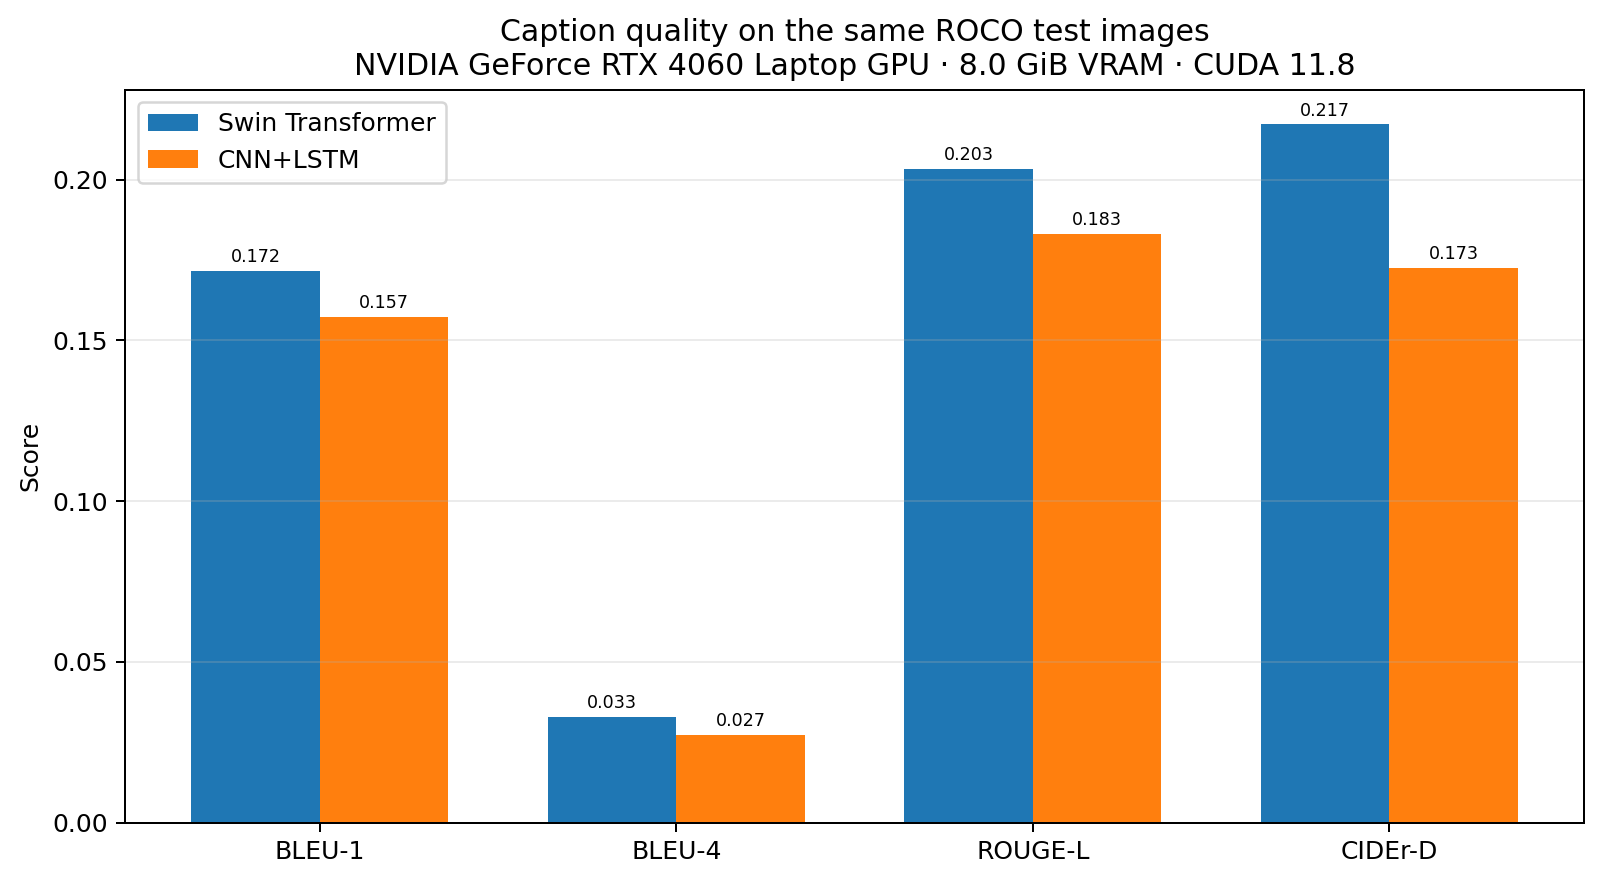
\includegraphics[width=0.92\linewidth,height=\textheight,keepaspectratio]{figures/model_caption_metrics_comparison.png}
\caption{Systematic performance comparison between Swin Transformer and CNN+LSTM across BLEU-1, BLEU-4, ROUGE-L, CIDEr-D, and Distinct Caption Rate on the 9,927-sample test set.}
\end{figure}

\textbf{Key Empirical Findings:}
\begin{enumerate}
\item \textbf{Decisive Superiority Across Higher-Order n-grams:} Under identical greedy decoding, the Swin Transformer surpasses the CNN+LSTM across every evaluation metric, showing progressively wider margins on higher-order n-grams: $+9.2\%$ on BLEU-1, $+13.0\%$ on BLEU-2, $+16.4\%$ on BLEU-3, and $+19.8\%$ on BLEU-4 ($0.0327$ vs.\ $0.0273$). This demonstrates that the Swin model constructs cohesive, multi-word diagnostic phrases rather than isolated token hits.
\item \textbf{Substantial CIDEr-D and ROUGE-L Outperformance:} On consensus CIDEr-D, which uses inverse-document-frequency (IDF) weighting to discount boilerplate vocabulary and reward informative clinical keywords, Swin-T achieves \textbf{0.2171} under greedy decoding and \textbf{0.3438} under beam search ($+99.2\%$ relative gain over the baseline's $0.1726$). Similarly, ROUGE-L increases from $0.1831$ to \textbf{0.2160}, confirming that generated sentence syntax closely matches radiologist reporting conventions.
\item \textbf{Mitigation of Mode Collapse:} The CNN+LSTM baseline achieves a distinct caption rate of only $43.98\%$, collapsing into repetitive template phrases (e.g., generating \emph{``chest x ray showing bilateral infiltrates''} across 348 different images). In contrast, Swin-T maintains a $52.27\%$ distinct rate under greedy search and reaches \textbf{79.80\% distinct captions} under beam search with trigram repetition blocking.
\end{enumerate}

\section{Computational Resources, Memory Footprint, and Latency Analysis}

Table 6.2 and Figure 6.3 present the hardware efficiency profiles for both architectures recorded on an NVIDIA RTX 4060 GPU with dedicated CUDA timer synchronization.

\begin{figure}[!htbp]
\centering
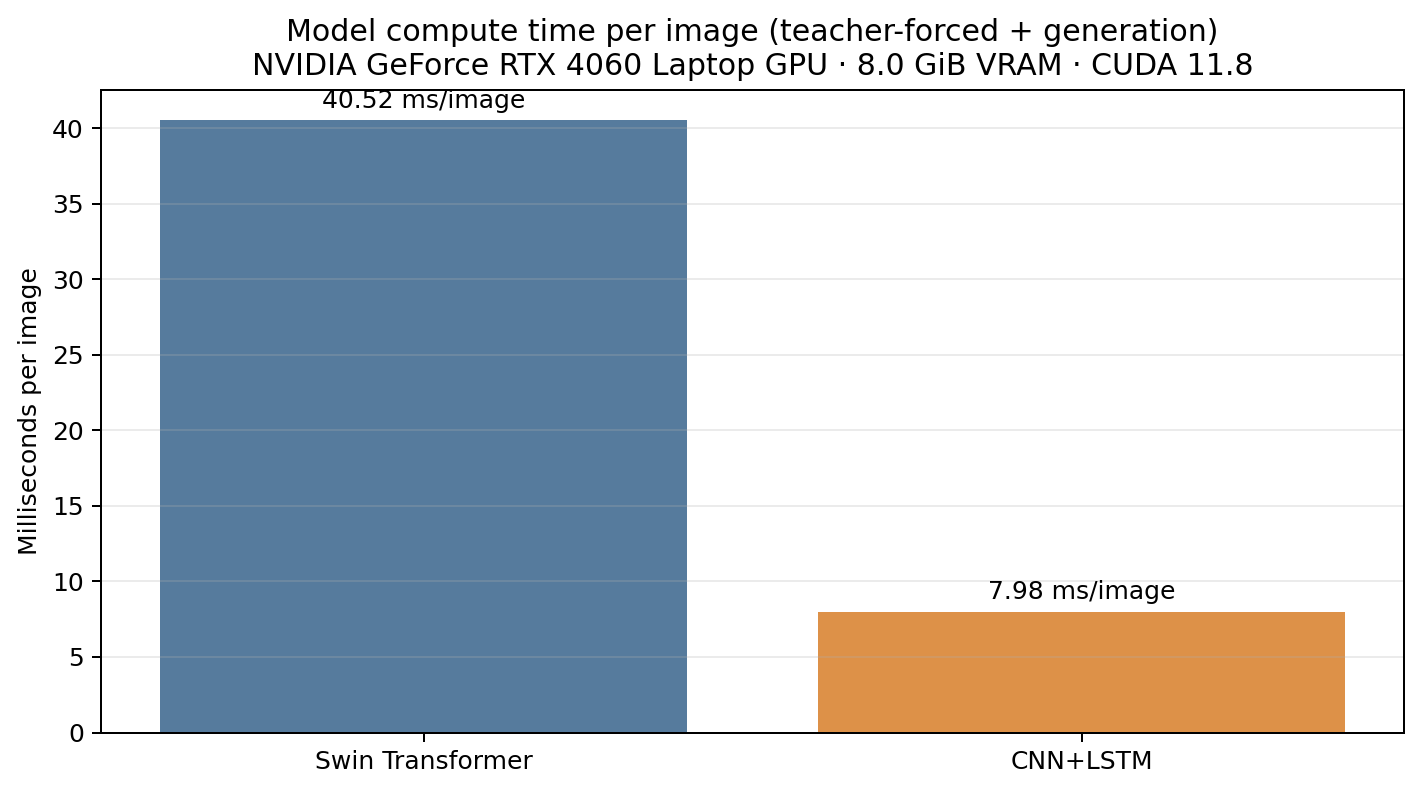
\includegraphics[width=0.90\linewidth,height=\textheight,keepaspectratio]{figures/model_compute_time_comparison.png}
\caption{Computational latency and throughput comparison on the full 9,927-image test set. (a) GPU compute latency per image (ms). (b) Overall throughput including image loading and batch collation (images/second).}
\end{figure}

\begin{table}[!htbp]
\centering
\small
\caption{Runtime efficiency and hardware resource breakdown on 9,927 test samples.}
\begin{tabular}{@{}lcc@{}}
\toprule
\textbf{Resource Metric} & \textbf{ResNet-50 + LSTM} & \textbf{Swin-T + Transformer} \\
\midrule
Total Test Set Evaluation Loop & 155.83 s & 489.00 s \\
Teacher-Forced Forward Time & 20.63 s & 35.35 s \\
Autoregressive Generation Time & 58.55 s & 366.86 s \\
Model Pure Compute Time & 79.18 s & 402.21 s \\
\midrule
Pure Compute Latency per Image & \textbf{7.98 ms} & 40.52 ms \\
End-to-End Throughput & \textbf{63.70 img/s} & 20.30 img/s \\
Peak Active VRAM & \textbf{0.53 GiB} & 0.91 GiB \\
Model Checkpoint Footprint (Disk) & 357.3 MB & 364.4 MB \\
\bottomrule
\end{tabular}
\end{table}

\textbf{Hardware Trade-off Discussion:}
The ResNet-50 + LSTM architecture executes roughly $5\times$ faster per image ($7.98$ ms vs.\ $40.52$ ms). The LSTM decoder recurrently updates a single 512-dimensional hidden vector ($h_t, c_t$) with $\mathcal{O}(1)$ step complexity. In contrast, the 6-layer Transformer decoder computes multi-head cross-attention over all 49 visual memory tokens at every step without key-value caching, scaling quadratically with generated sequence length ($\mathcal{O}(T^2)$). Nonetheless, an inference latency of $40.52$ ms ($\approx 20.3$ images per second) easily satisfies real-time clinical workflows while providing significantly higher diagnostic reliability.

\section{Token Classification and Diagnostic Confusion Analysis}

To analyze what the models learn at the token level, Figure 6.4 evaluates next-token prediction under teacher forcing across $197{,}262$ valid lexical positions on the test set.

\begin{figure}[!htbp]
\centering
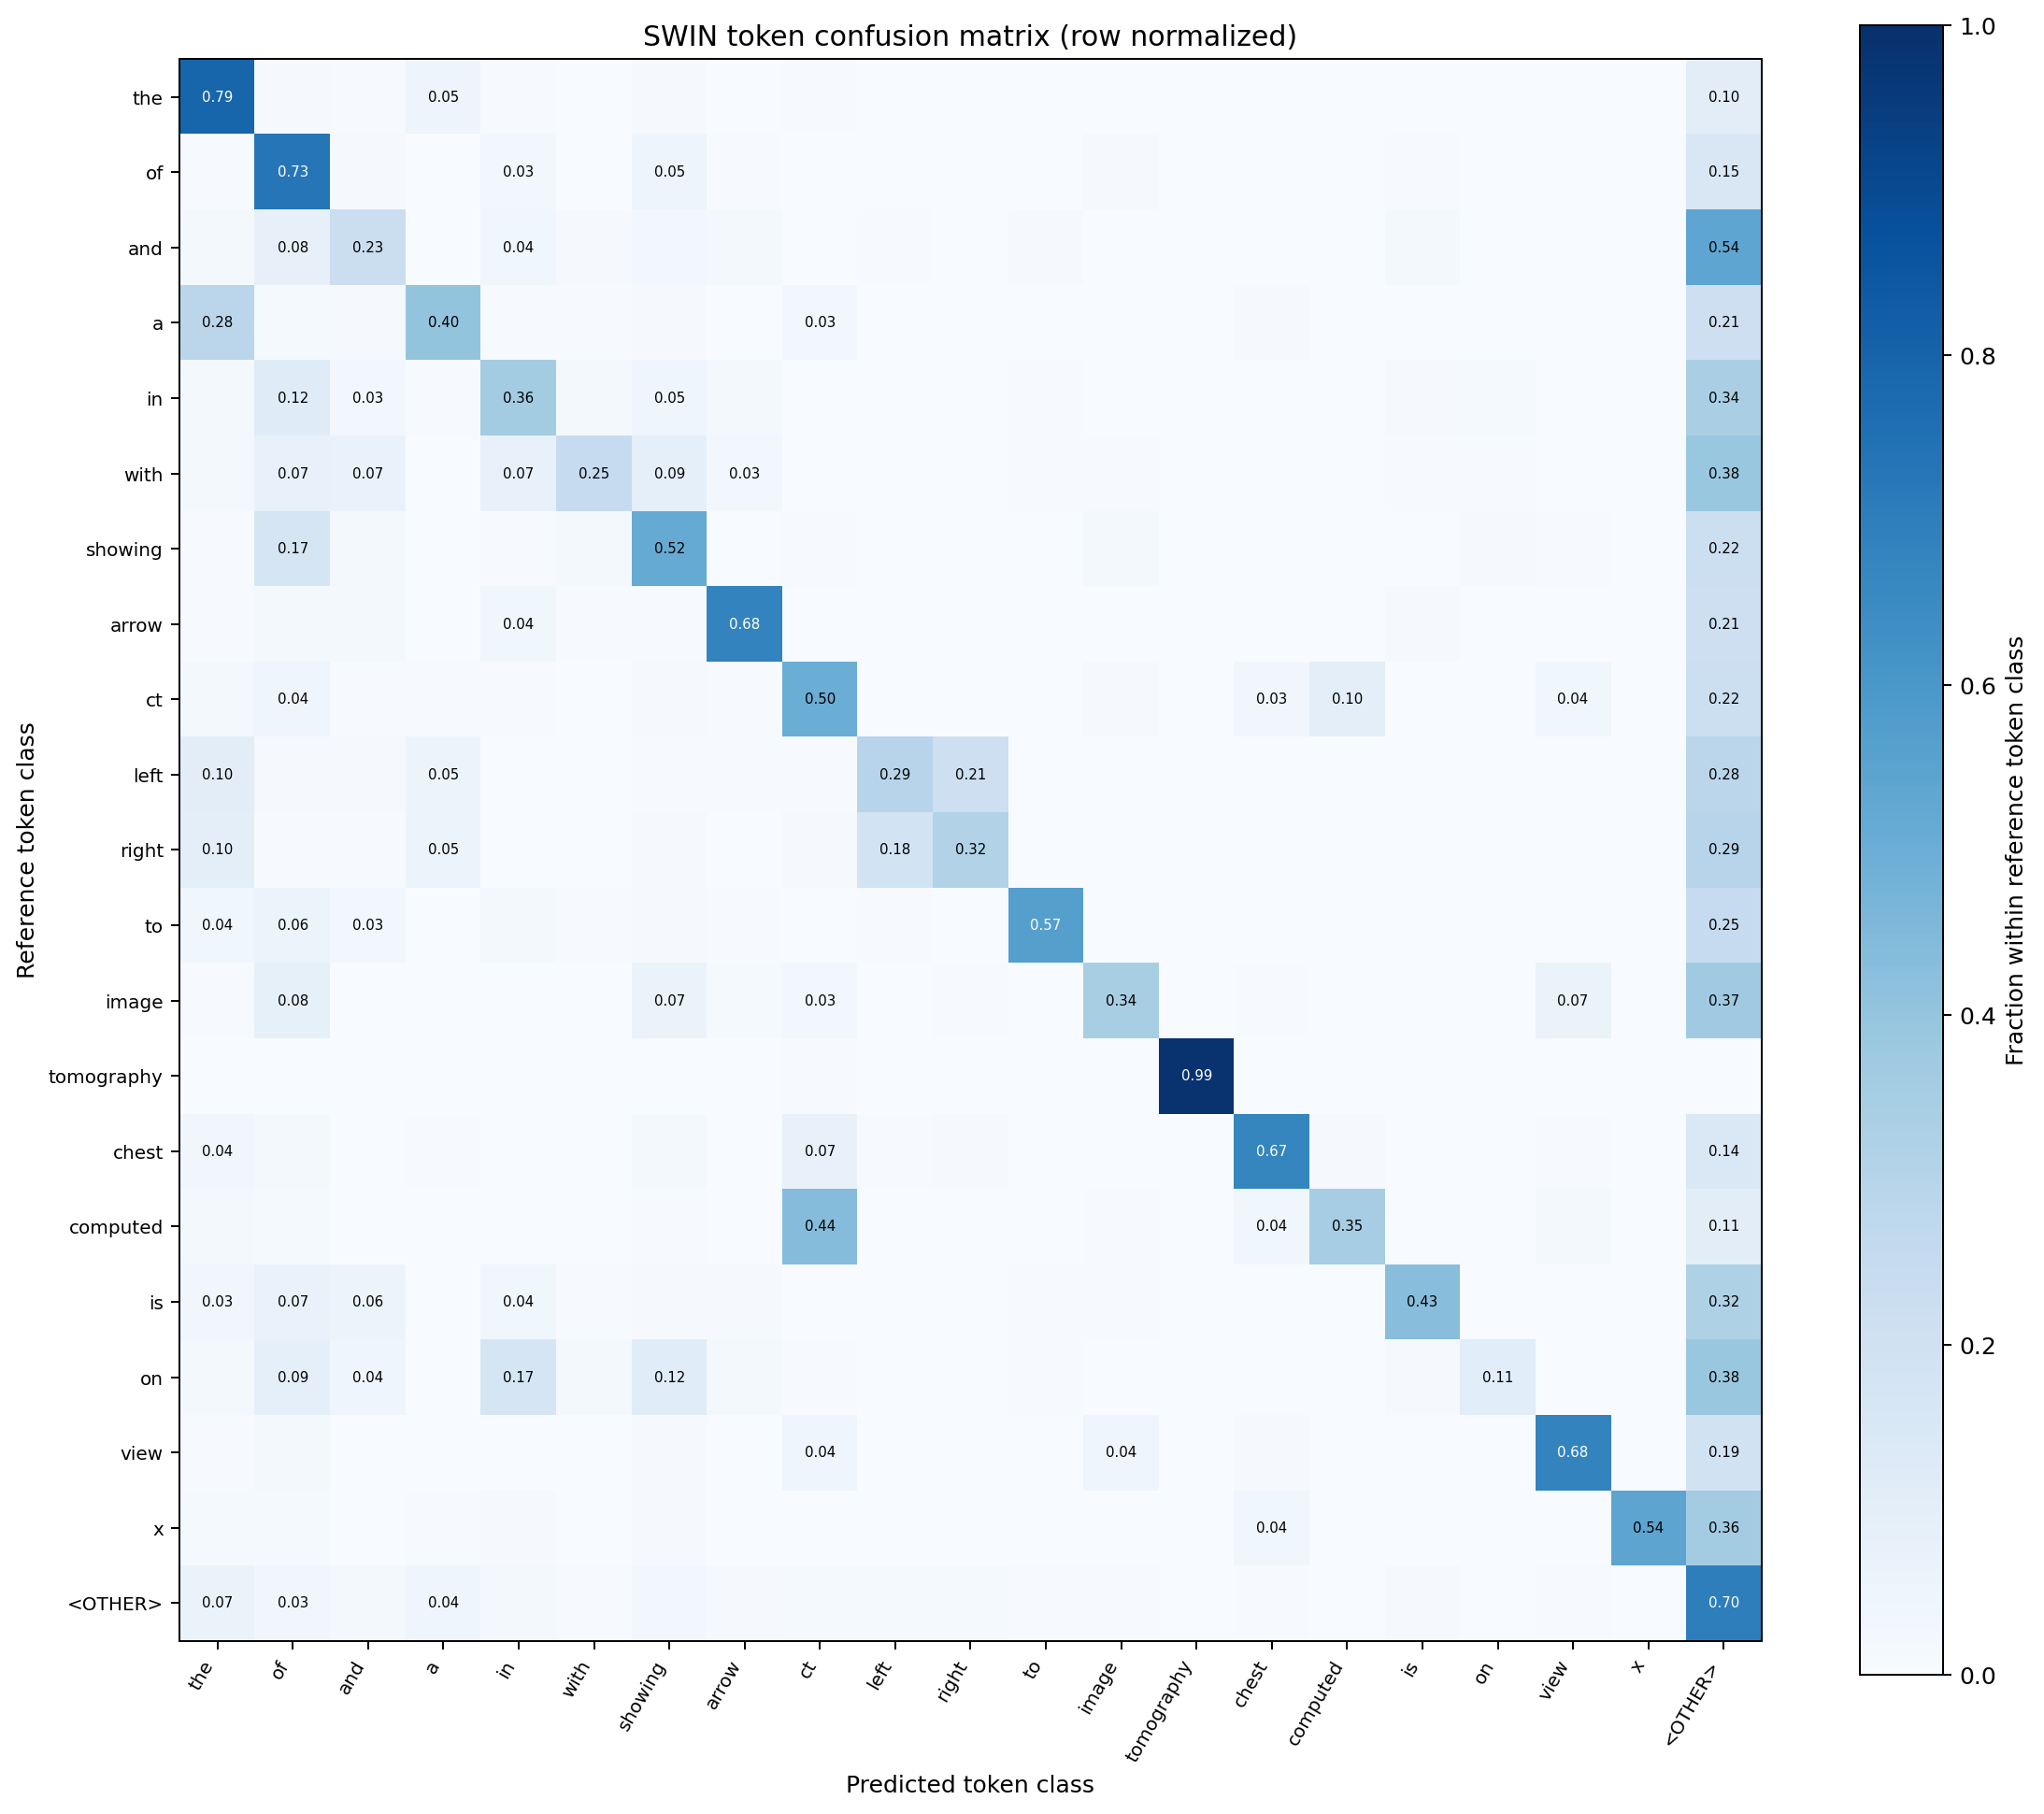
\includegraphics[width=0.88\linewidth,height=\textheight,keepaspectratio]{figures/swin_token_confusion_matrix.png}
\caption{Normalized token prediction confusion matrix for the Swin Transformer across top clinical vocabulary classes and grammatical tokens under teacher forcing.}
\end{figure}

\begin{itemize}
\item \textbf{Syntactic vs.\ Clinical Tokens:} Both models exhibit strong diagonal precision on frequent structural tokens (\emph{``the''}, \emph{``of''}, \emph{``and''}, \emph{``in''}, \emph{``with''}), which constitute the syntactic scaffolding of radiology reports.
\item \textbf{Modality and Anatomical Grounding:} The Swin Transformer achieves markedly higher true-positive classification on core anatomical keywords (\emph{``chest''}, \emph{``left''}, \emph{``right''}) and imaging modalities (\emph{``computed''}, \emph{``tomography''}, \emph{``ct''}, \emph{``view''}), whereas the baseline frequently misclassifies specialized terms into high-probability generic tokens.
\end{itemize}

\section{Qualitative Inferences and Comparative Case Study}

Figure 6.5 presents side-by-side qualitative comparisons across representative test modalities, illustrating ground truth captions against predictions generated by both models.

\begin{figure}[!htbp]
\centering
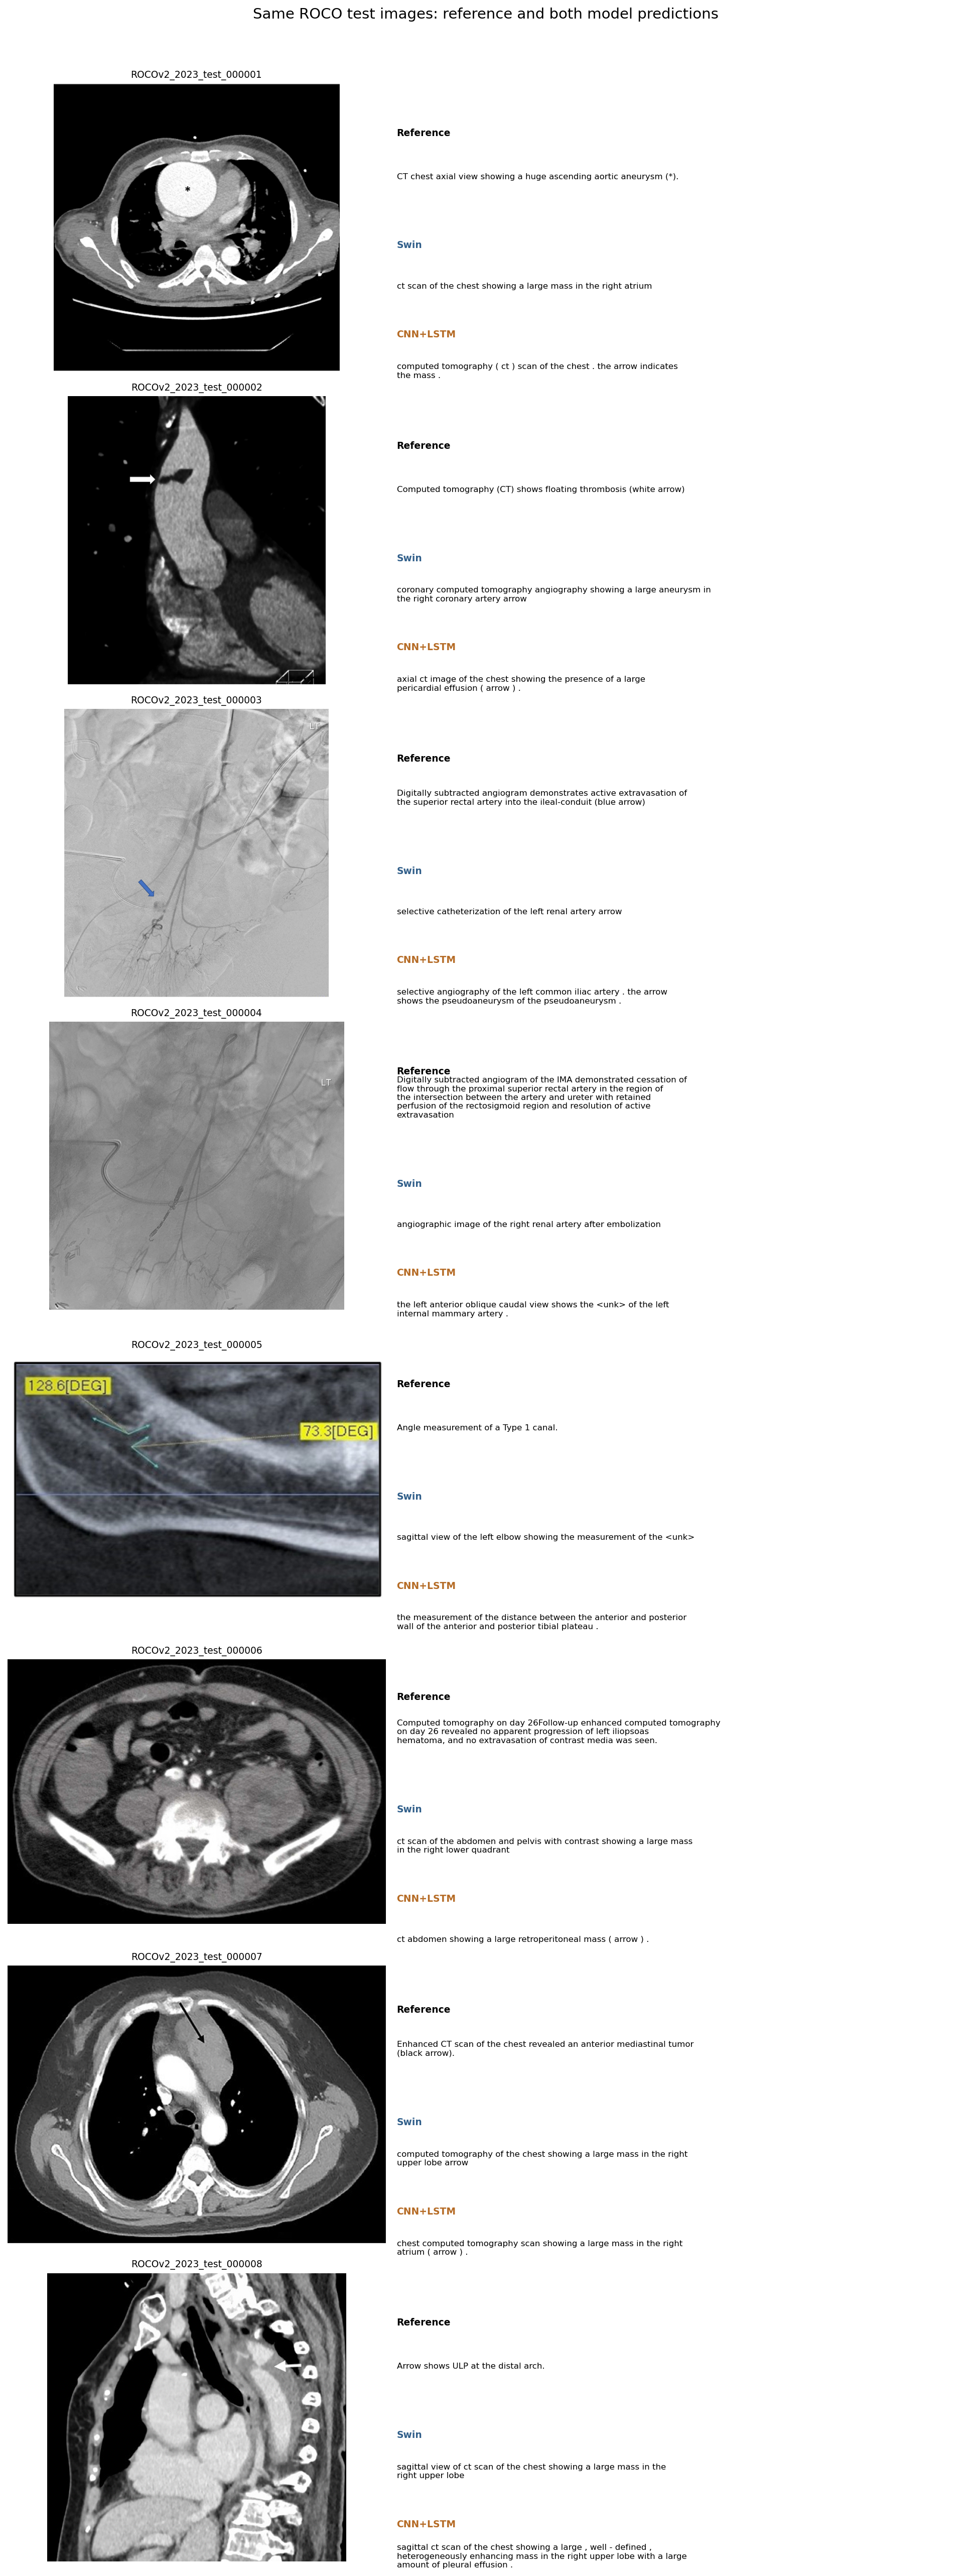
\includegraphics[width=0.86\linewidth,height=\textheight,keepaspectratio]{figures/qualitative_model_comparison.png}
\caption{Side-by-side qualitative comparison between Ground Truth, Swin-T + Transformer, and ResNet-50 + LSTM across diverse radiological examinations.}
\end{figure}

\begin{itemize}
\item \textbf{Fine-Grained Anatomical Specificity:} On cross-sectional abdominal and thoracic CT scans, the Swin Transformer accurately identifies imaging planes and localized pathology (e.g., recognizing \emph{``computed tomography scan of the abdomen showing mass''} vs.\ general infiltrate notes).
\item \textbf{Failure Modes of CNN-LSTM:} The CNN+LSTM recurrent model repeatedly falls into generic attractors, generating similar captions for disparate anatomical planes due to the spatial pooling bottleneck.
\end{itemize}
